  %%%%%%%%%%%%%%%%%%%%%%%%%%%%%%%%%%%%%%%%%
% Daily Laboratory Book
% LaTeX Template
%
% This template has been downloaded from:
% http://www.latextemplates.com
%
% Original author:
% Frank Kuster (http://www.ctan.org/tex-archive/macros/latex/contrib/labbook/)
%
% Important note:
% This template requires the labbook.cls file to be in the same directory as the
% .tex file. The labbook.cls file provides the necessary structure to create the
% lab book.
%
% The \lipsum[#] commands throughout this template generate dummy text
% to fill the template out. These commands should all be removed when
% writing lab book content.
%
% HOW TO USE THIS TEMPLATE
% Each day in the lab consists of three main things:
%
% 1. LABDAY: The first thing to put is the \labday{} command with a date in
% curly brackets, this will make a new page and put the date in big letters
% at the top.
%
% 2. EXPERIMENT: Next you need to specify what experiment(s) you are
% working on with an \experiment{} command with the experiment shorthand
% in the curly brackets. The experiment shorthand is defined in the
% 'DEFINITION OF EXPERIMENTS' section below, this means you can
% say \experiment{pcr} and the actual text written to the PDF will be what
% you set the 'pcr' experiment to be. If the experiment is a one off, you can
% just write it in the bracket without creating a shorthand. Note: if you don't
% want to have an experiment, just leave this out and it won't be printed.
%
% 3. CONTENT: Following the experiment is the content, i.e. what progress
% you made on the experiment that day.
%
%%%%%%%%%%%%%%%%%%%%%%%%%%%%%%%%%%%%%%%%%

%----------------------------------------------------------------------------------------
%	PACKAGES AND OTHER DOCUMENT CONFIGURATIONS
%----------------------------------------------------------------------------------------

\documentclass[idxtotoc,hyperref,openany]{labbook} % 'openany' here removes the gap page between days, erase it to restore this gap; 'oneside' can also be added to remove the shift that odd pages have to the right for easier reading
\usepackage{amsmath}
\usepackage[
  backref=page,
  pdfpagelabels=true,
  plainpages=false,
  colorlinks=true,
  bookmarks=true,
  pdfview=FitB]{hyperref} % Required for the hyperlinks within the PDF
\usepackage{hyperref}
\usepackage{listings}
\usepackage{booktabs} % Required for the top and bottom rules in the table
\usepackage{float} % Required for specifying the exact location of a figure or table
\usepackage{graphicx} % Required for including images
\usepackage{lipsum} % Used for inserting dummy 'Lorem ipsum' text into the template
\usepackage{colortbl}
\usepackage{cite}
\usepackage{bm}
\usepackage{subcaption}
\usepackage{mwe}
\usepackage{multirow}
\usepackage[normalem]{ulem}
\usepackage{amsmath,amsfonts,amsthm} % Math packages
\newcommand{\HRule}{\rule{\linewidth}{0.5mm}} % Command to make the lines in the title page
\setlength\parindent{0pt} % Removes all indentation from paragraphs
\setcounter{MaxMatrixCols}{20}
%----------------------------------------------------------------------------------------
%	DEFINITION OF EXPERIMENTS
%----------------------------------------------------------------------------------------
\usepackage{color}

\definecolor{mygreen}{rgb}{0,0.6,0}
\definecolor{mygray}{rgb}{0.5,0.5,0.5}
\definecolor{mymauve}{rgb}{0.58,0,0.82}

\lstset{ 
  backgroundcolor=\color{white},   % choose the background color; you must add \usepackage{color} or \usepackage{xcolor}; should come as last argument
  basicstyle=\footnotesize,        % the size of the fonts that are used for the code
  breakatwhitespace=false,         % sets if automatic breaks should only happen at whitespace
  breaklines=true,                 % sets automatic line breaking
  captionpos=b,                    % sets the caption-position to bottom
  commentstyle=\color{mygreen},    % comment style
  deletekeywords={...},            % if you want to delete keywords from the given language
  escapeinside={\%*}{*)},          % if you want to add LaTeX within your code
  extendedchars=true,              % lets you use non-ASCII characters; for 8-bits encodings only, does not work with UTF-8
  frame=single,	                   % adds a frame around the code
  keepspaces=true,                 % keeps spaces in text, useful for keeping indentation of code (possibly needs columns=flexible)
  keywordstyle=\color{blue},       % keyword style
  language=Octave,                 % the language of the code
  morekeywords={*,...},            % if you want to add more keywords to the set
  numbers=left,                    % where to put the line-numbers; possible values are (none, left, right)
  numbersep=5pt,                   % how far the line-numbers are from the code
  numberstyle=\tiny\color{mygray}, % the style that is used for the line-numbers
  rulecolor=\color{black},         % if not set, the frame-color may be changed on line-breaks within not-black text (e.g. comments (green here))
  showspaces=false,                % show spaces everywhere adding particular underscores; it overrides 'showstringspaces'
  showstringspaces=false,          % underline spaces within strings only
  showtabs=false,                  % show tabs within strings adding particular underscores
  stepnumber=2,                    % the step between two line-numbers. If it's 1, each line will be numbered
  stringstyle=\color{mymauve},     % string literal style
  tabsize=2,	                   % sets default tabsize to 2 spaces
  title=\lstname                   % show the filename of files included with \lstinputlisting; also try caption instead of title
}
\newexperiment{example}{This is an example experiment}
\newexperiment{example2}{This is another example experiment}
\newexperiment{example3}{This is yet another example experiment}
\newexperiment{table}{This shows a sample table}
%\newexperiment{shorthand}{Description of the experiment}

%---------------------------------------------------------------------------------------

\begin{document}
\tableofcontents
\chapter{Hummingbird}
This chapter describes how to control the Hummingbird quadrotor. Fig. \ref{fig_hummingbird} shows the experimental setup for the time-optimal landing of a quadrotor onto a moving platform. The setup includes a computer which runs the controller, the motion capture system and the Hummingbird quadrotor. This chapter will introduce each parts in detail. 

\begin{figure}
\centering
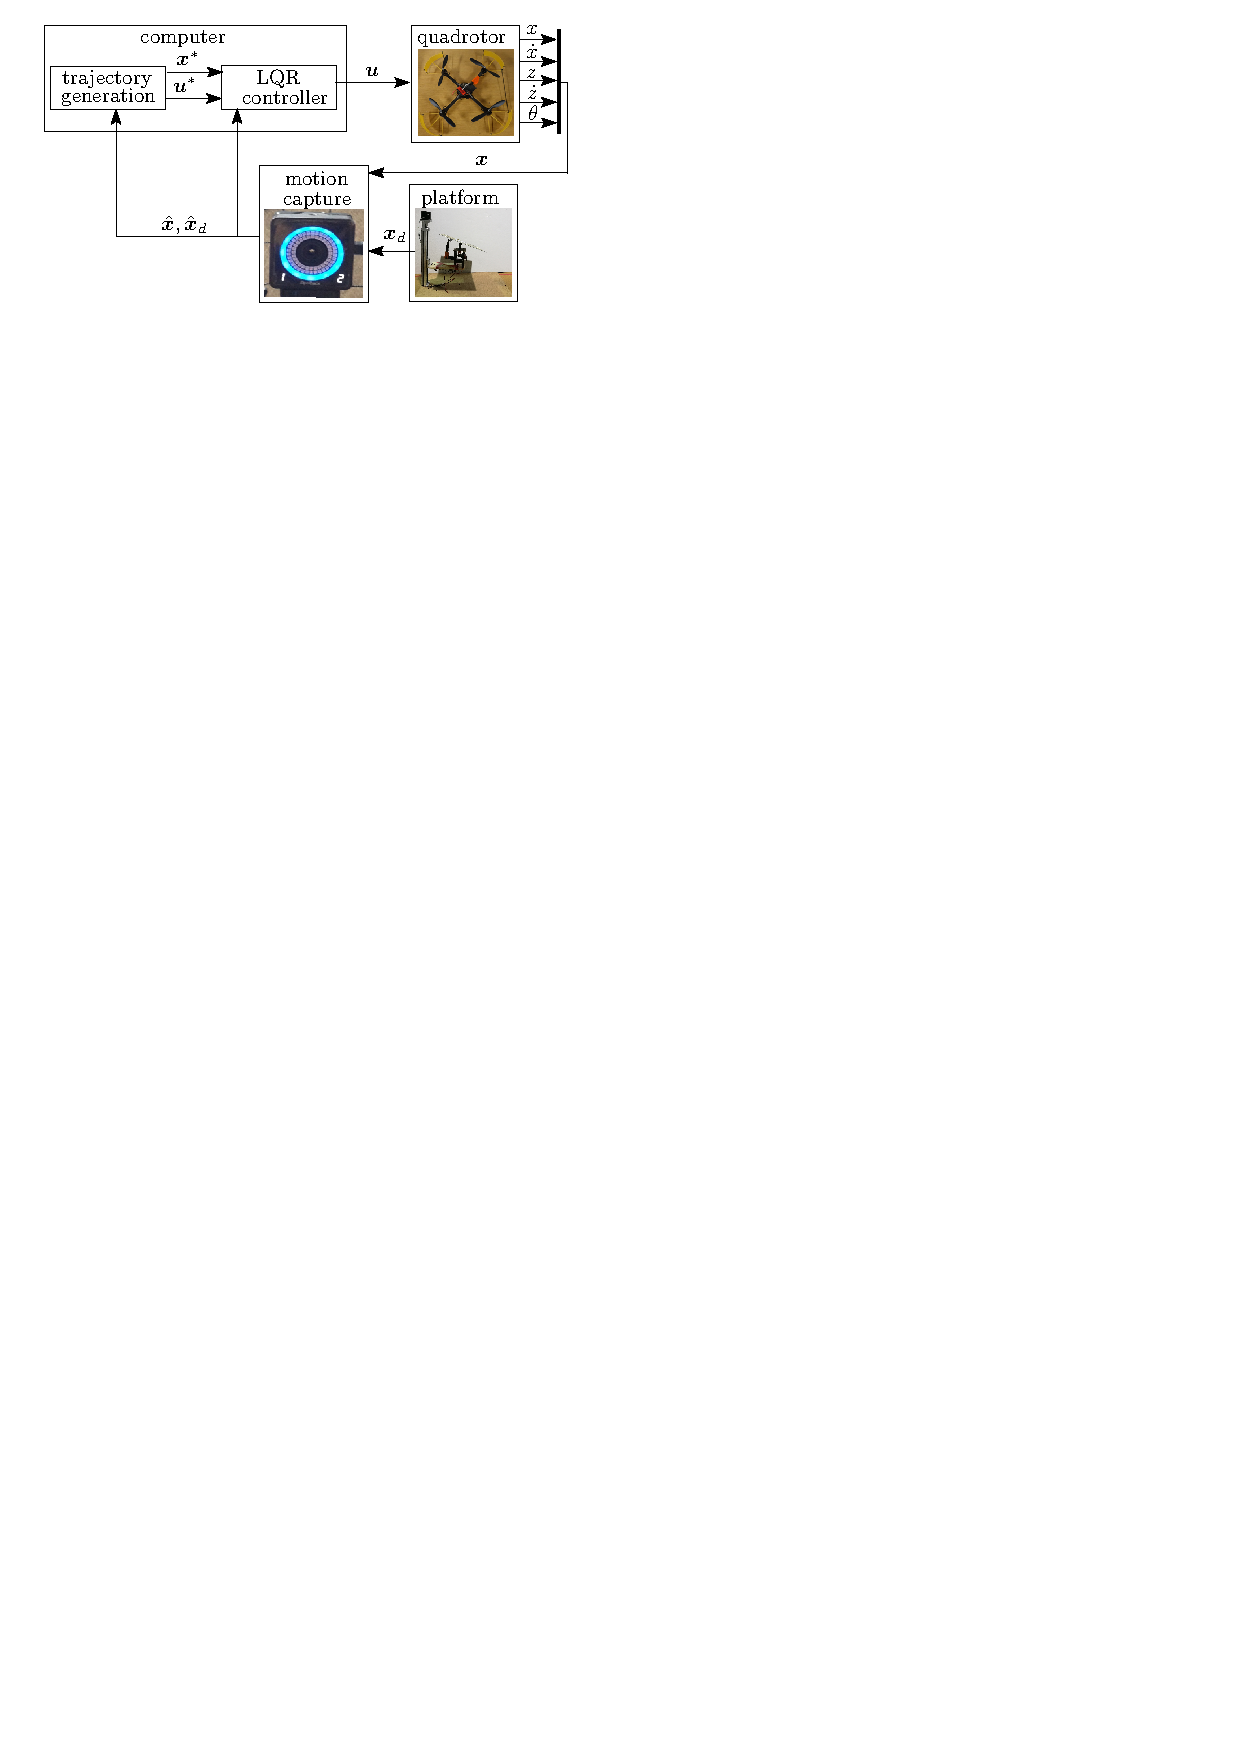
\includegraphics[scale=1]{./Figure/fig_ExperimentalSetup}
\caption{Figure of the experimental setup for quadrotor landing onto a heaving platform}\label{fig_hummingbird}
\end{figure}
\section{Motion capture system}

To use the motion capture system, there are several steps.

\begin{enumerate}
\item Turn on the Windows desktop.  The \textbf{user name} is: Young. The \textbf{password} is: andrew.
\item Click on the Motion capture software. 
\item Turn on the power of the motion capture system. There is a power extension cord on the ground. If the power is on, the motion capture cameras can be seen in the motion capture software as shown in Fig. \ref{fig_motioncapfront}. The blue LEDs on several motion capture cameras are turned on. 

\begin{figure}
\centering
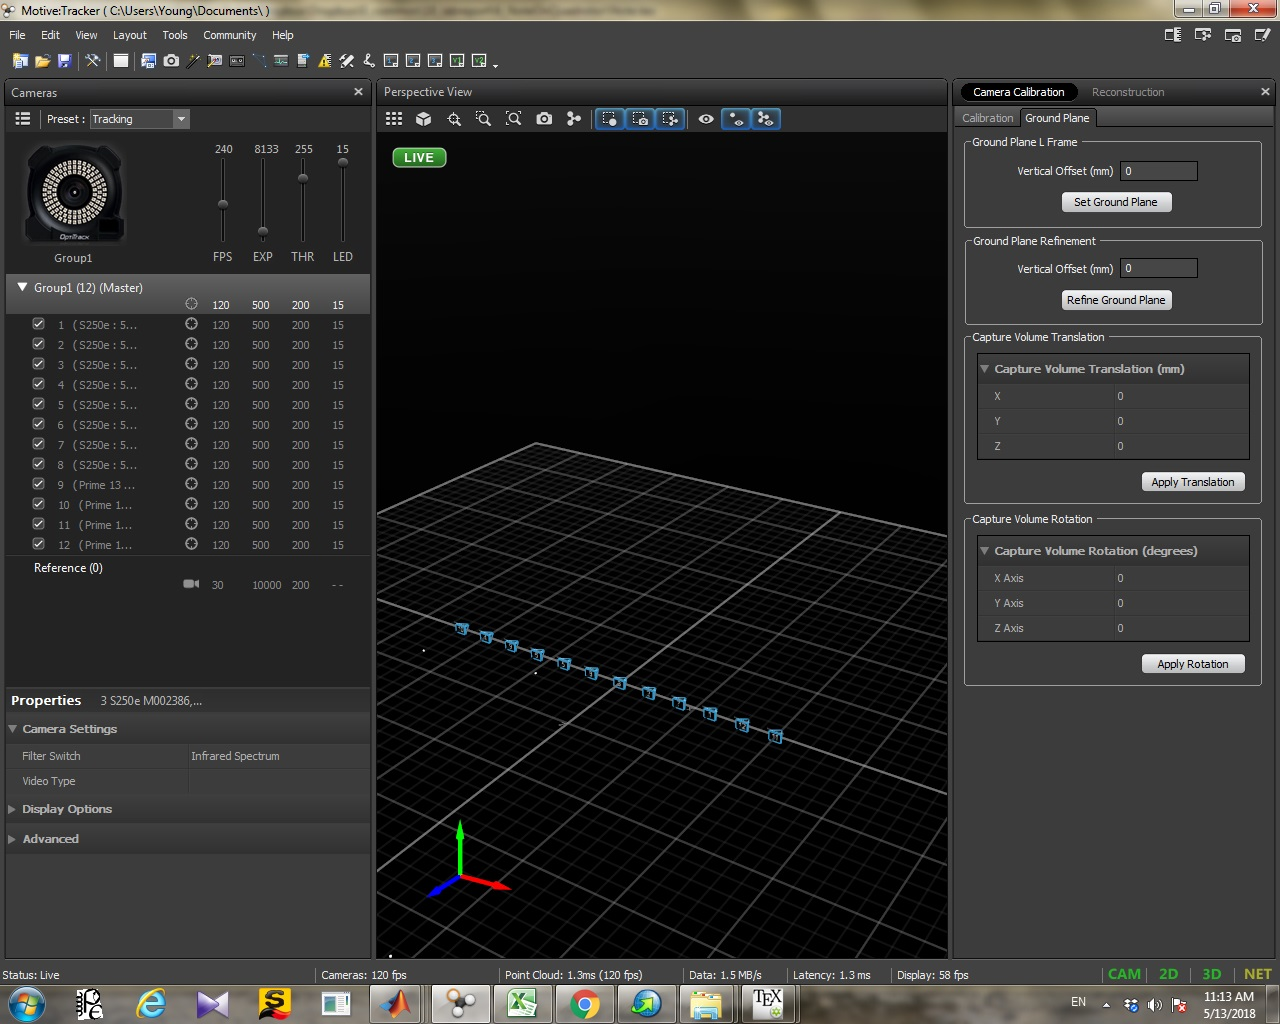
\includegraphics[scale=0.2]{./Figure/fig_MotioncapFront}
\caption{Figure of the front panel of the motion capture software}\label{fig_motioncapfront}
\end{figure}
\item Click on ``File-$>$Open", select the camera calibration file (the postfix is *.cal). If there are extra white dots in the field, these are noise points that should be filtered. In this case, click on ``View-$>$Camera Calibration-$>$Mask Visible". The white nose dots will be filtered out.  
\item Put the quadrotor on the ground. From the motion capture software, it can be seen four white markers. Select four markers, then right click. Click ``Rigid body-$>$Created from selected markers". The default coordinate of the motion capture system is defined in Fig. \ref{fig_lablayout}. The positive $x$ direction on the quadrotor is defined as shown in Fig. \ref{fig_quadrotor}. It is necessary that the $x$ direction of the quadrotor matches the $x$ direction of the motion capture system.
\begin{figure}[h!]
\centering
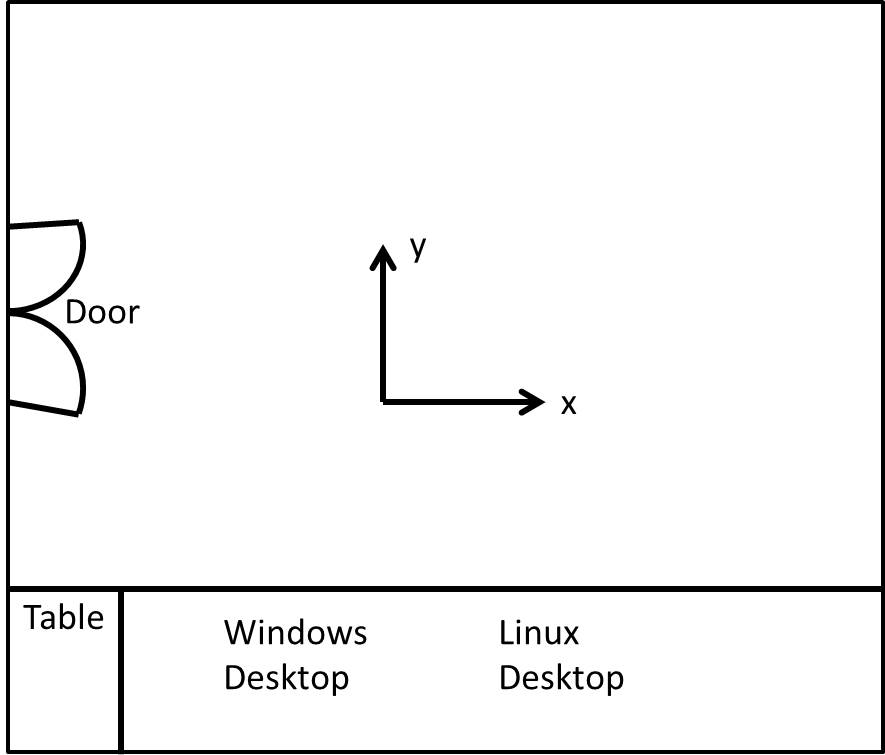
\includegraphics[scale=0.3]{./Figure/fig_lablayout}
\caption{Figure of the lab layout. The $z$ direction is pointing upward.}\label{fig_lablayout}
\end{figure}
\begin{figure}[h!]
\centering
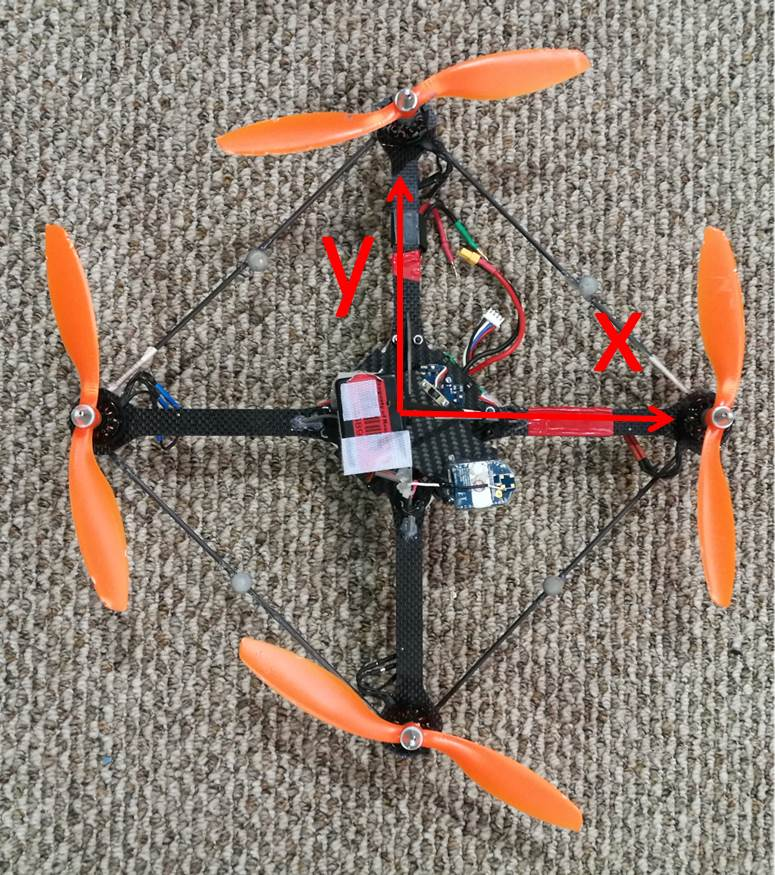
\includegraphics[scale=0.3]{./Figure/fig_quadrotor}
\caption{Figure of the quadrotor direction. The arm with a long red tape is the $x$ direction.}\label{fig_quadrotor}
\end{figure}

\item Right click in the middle point of the rigid body, select ``Properties". Change the name to be ``Tracker0". The first letter ``T" must be capitalized to be consistent with the definition on the Linux desktop.
\item Click on ``View-$>$Data Stream", check the box for ``Broadcast Frame Data" under the ``VRPN Streaming Engine". This is to broadcast the data for the Linux desktop. To broadcast the data on the Windows system, check the box for  ``Broadcast Frame Data" under the ``OptiTrack Streaming Engine". 
\end{enumerate} 



\subsection{Motion capture system on Windows system}
After setting up the motion capture software, there are several steps to receive command on the Windows desktop. 

\begin{enumerate}
\item Open Matlab. 
\item Open the example code folder. After running the code, it can be seen that the position and angles of the quadrotor are plotted. 
\end{enumerate}
\subsection{Motion capture system on Linux system}
After setting up the motion capture software, there are several steps to receive command on the Linux desktop. 

\begin{enumerate}
\item Open the Linux desktop. The \textbf{user name} is: botao, the \textbf{password} is: hub20417.
\item Open the Matlab. Currently the Motion Capture software is supported on the Matlab 2014. To install the Motion Capture support on newer version of Matlab, please refer to the installation of vrpn located in the folder. To open the Matlab 2014, click on Documents-$>$Matlab-$>$bin. Then right click on the screen, select ``open terminal" and input following command:
\begin{lstlisting}[language=bash]
>>./matlab
\end{lstlisting}
\item Connect the green Ethernet cable onto the Linux desktop and select the connection to be ``Motion capture". 
\item Go to the template folder and run the code. The position and angle should be able to be printed.  
\end{enumerate}
\subsection{Frequent mistakes}
\begin{enumerate}
\item The motion capture connection is lost. 

Answer: This happens when the power of the motion capture system is lost or the motion capture software has been restarted.  The Matlab will usually not complain but the position and Euler angles of the quadrotor will not be updated. If the quadrotor flies in this situation, the quadrotor will crash because the feedback is lost. The way to detect this mistake is to compute the variance of the motion capture data. If the variance is zero, then it indicates that the connection has been lost and the Matlab will need to be restarted. 
\item The Matlab complains no connection.

Answer: This happens when the connection is not correctly set. The way to solve this problem is to double check the connection, especially the Ethernet connection, the stream broadcast, the Ethernet cable connection.

\item Why we are using the Linux system?

Answer: The connection between the desktop and Hummingbird has only been verified on the Linux system. The detail on how to control the Hummingbird quadrotor will be described later. 

\item How to perform motion capture camera calibration?

Answer: Please refer to the manual for the camera calibration (\url{https://v20.wiki.optitrack.com/index.php?title=Calibration}). It should be noticed that the camera calibration must be performed after one or more cameras have changed location or orientation. 
\end{enumerate}

\newpage
\section{Computer}
\subsection{Computer setup}
To control the quadrotor, there are several steps.

\begin{enumerate}
\item Turn on the quadrotor.
\item Turn on the joystick.
\item Hold the left joystick to the bottom left until the motors are spinning as shown in Fig. \ref{fig_joystick}. Make sure that the joystick has enough voltage (above 11.1 v). If the voltage is less than 11.1 Volt, it is necessary to switch the battery. Currently the battery is rechargeable. 

\begin{figure}[h!]
\centering
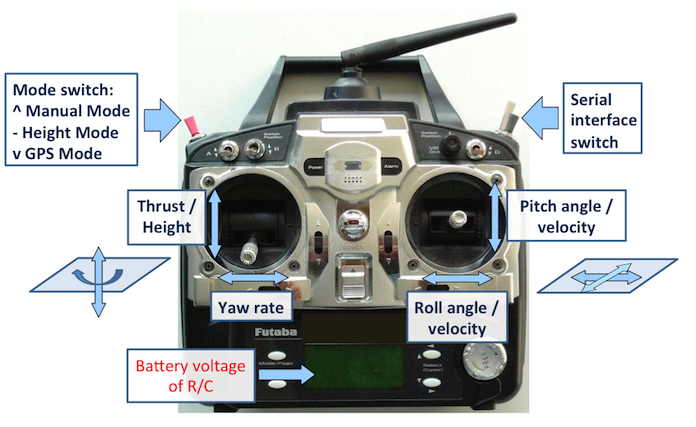
\includegraphics[scale=0.3]{./Figure/fig_joystick}
\caption{Figure of the joystick for Hummingbird control. A detail introduction can be found at Ascending Technology website (\url{http://wiki.asctec.de/display/AR/Get+Ready+to+Fly}).}\label{fig_joystick}
\end{figure}
\item Connect the Zigbee to the desktop. Make sure the Zigbee plugged in has the label Hummingbird on the top as shown in Fig. \ref{fig_zigbee}.
\begin{figure}[h!]
\centering
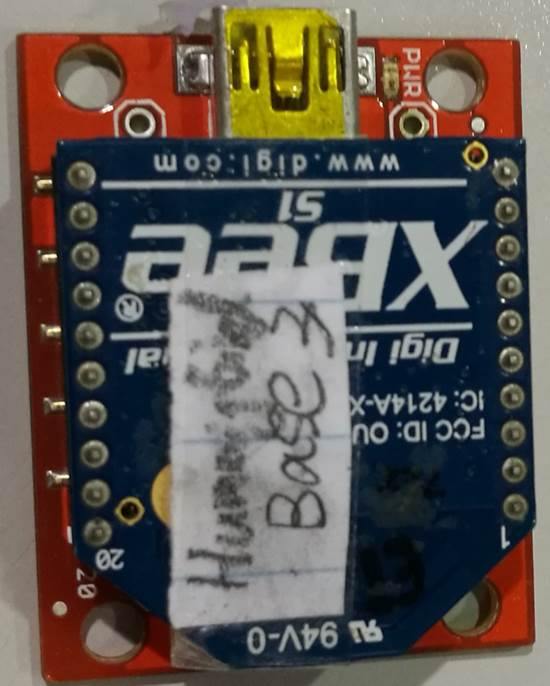
\includegraphics[scale=0.3]{./Figure/fig_zigbee}
\caption{Figure of the zigbee for the Hummingbird control.}\label{fig_zigbee}
\end{figure}
\item On the Linux  computer, go to the folder and runs the following command:
\begin{lstlisting}[language=bash]
./aci_command 4773
\end{lstlisting}

It should display the following information:
\begin{lstlisting}[language=bash]
Waiting for command list ...
command list getted!
running speed 0

\end{lstlisting}
\item Toggle the  ``serial interface switch" on the joystick (shown in Fig. \ref{fig_joystick}) and the motors should stop spinning.
\item Open the Matlab folder, runs the function. It should pop out a Graphical User Interface. The variance should be displayed. If the variances are all zero, then check the connection of the motion capture system. If the variances are not zero, click ``Start" on the user interface. 
\item Move the joystick, the quadrotor should be able to follow the joystick motion.
\item In any emergency situation, click ``Stop" on the user interface, the motors should stop spinning.
\end{enumerate}


\subsection{Frequent problem}
\begin{enumerate}
\item The information does not display. It only display the following information:
\begin{lstlisting}[language=bash]
Waiting for command list...
\end{lstlisting}

Answer: It could be caused by the fact that the connection between the Hummingbird and the desktop has not been established. In this case, try to restart the terminal and the Hummingbird。
\item The information displays successfully and  the ``serial interface switch" has been switched but the motors keep running

Answer: It could be caused by the fact that the USB port is not correctly set. Open the terminal and type in the following command:
\begin{lstlisting}[language=bash]
ls /dev/ttyUSB*
\end{lstlisting}

Open the main.c file and change the line to the correct port number. 

\begin{lstlisting}[language=bash]
fd = open("/dev/ttyUSB0", O_RDWR | O_NOCTTY | O_NDELAY | O_NONBLOCK);
\end{lstlisting}

Then it is important to remake the folder. At the terminal, runs the following code:
\begin{lstlisting}[language=bash]
>>make
\end{lstlisting}


It could also be caused by the fact that a wrong Zigbee is plugged in. Make sure the Zigbee plugged in has a label (Zigbee) on the top. 

\item How to set up the Zigbee?

Answer: Please following the instructions on the following website: \url{http://wiki.asctec.de/display/AR/XBee+Modules}. To pair the Zigbee module on the Hummingbird, the Zigbee channel is D, the PAN ID is 2. The destination low is 2 and the 16 bit source address is 20. 

\item Where does the number ``4773" come from?

Answer: It is the channel number that communicates between the Matlab and the aci$\_$command code. The same number is used in the Matlab script.

\begin{lstlisting}[language=Matlab]
port=4773; 
t=tcpip('localhost',port);
fopen(t);
\end{lstlisting}

\item There is an error message when trying to run the ``aci\textunderscore command":
\begin{lstlisting}[language=bash]
Waiting for command list...
command list getted!
running speed 0
./aci_command: Segmentation fault (core dumped)
\end{lstlisting}

Answer: this is caused by the fact there is a connection conflict. It usually happens when the last session is not closed properly. Usually there are two ways to deal with this problem. The first one is to restart the computer. The second one is change the channel number. For example, try to run the following command:
\begin{lstlisting}[language=bash]
./aci_command 4774
\end{lstlisting}

The code in the Matlab function should also be changed accordingly
\begin{lstlisting}[language=Matlab]
port=4774; 
t=tcpip('localhost',port);
fopen(t);
\end{lstlisting}
\end{enumerate}


\newpage
\section{Hummingbird quadrotor}

The website for the Hummingbird can be found at the following website:

\url{http://wiki.asctec.de/display/AR/AscTec+Hummingbird}

Please note that the product is not longer supported by Intel. 
\subsection{Quadrotor setup}
The $x$ axis of the quadrotor should be placed with the same direction as the motion capture system as shown in Fig. \ref{fig_quadrotor}.

To turn on the quadrotor, there are two steps.
\begin{enumerate}
\item Plug in the battery. Make sure that the positive and negative wires are connected correctly. 
\item Turn on the motor. It should beep a few times and be quite. A detail of the acoustic feedback can be found at \url{http://wiki.asctec.de/display/AR/Acoustic+Feedback}. The common patterns are shown in Fig. \ref{fig_acoustic}.
\end{enumerate}


\begin{figure}[h!]
\centering
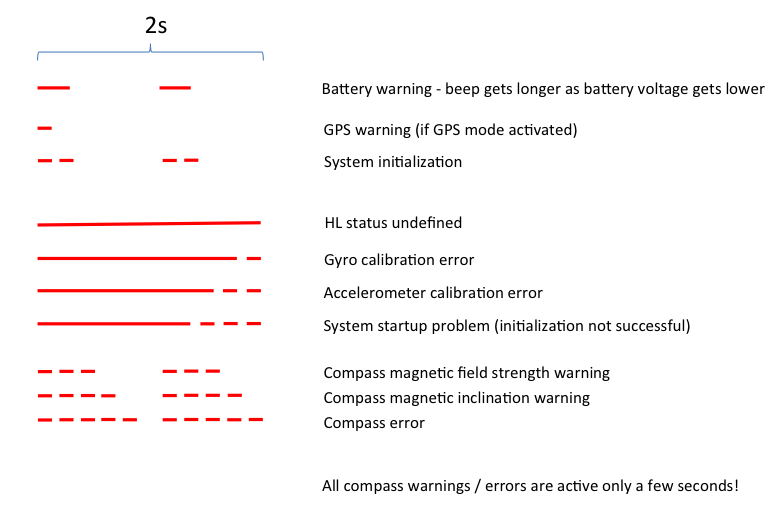
\includegraphics[scale=0.5]{./Figure/Acoustic}
\caption{Figure of acoustic feedback}\label{fig_acoustic}
\end{figure}

\subsection{Battery}
 
Currently a 1400mAh Lipo battery is used for the Hummingbird. It is important that the battery is not over discharged otherwise it will cause permanent damage to the battery. It is very dangerous therefore not recommended to charge an over discharged battery.

To prevent over discharging a battery, it is important to keep an eye on the voltage of the battery and charge the battery before the voltage drops below 11.1 vol. The voltage meter (shown in Fig. \ref{fig_battery}) is used to measure the voltage of a Lipo battery. It is very \textbf{important to remove the voltage meter after using it}. The voltage meter will consume current and if it is left on the battery for one night, the battery will be over discharged and can not be used anymore. 

\begin{figure}
\centering
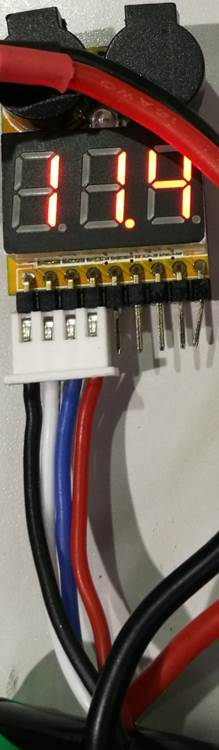
\includegraphics[scale=0.4]{./Figure/fig_battery}
\caption{Figure of voltage meter connection to the Lipo battery}\label{fig_battery}
\end{figure}


To charge the battery, please following the following steps:

\begin{enumerate}
\item Connect the battery to the charge as shown in Fig. \ref{fig_charge}. It is important to connect the voltage balance.
\item Open the power supply. Change the voltage output to be 24V.
\item Select the capacity to be 1400mAh (\textbf{same as the battery}), long press the enter. Then it will begin to charge. 
\item When the charging process is finished, the charger will beep. Just turn off the power supply and remove the battery. 
\end{enumerate}

\begin{figure}
\centering
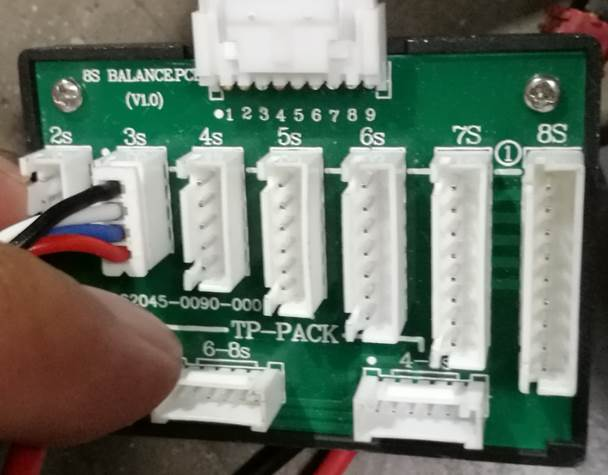
\includegraphics[scale=0.5]{./Figure/fig_charge}
\caption{Figure of battery charger.}\label{fig_charge}
\end{figure}
\subsection{Frequent questions}
\begin{enumerate}
\item Can the Hummingbird controlled on a Windows laptop?

Answer: For now it is difficult. It needs to run the ``aci$\_$command" function to build the connection between the Hummingbird and the desktop. I have not tried to implement the code on a Windows computer but I assume it is possible. 

\item Can the update rate for the Hummingbird increased?

Answer: Currently the control command is sent wirelessly through Zigbee at a rate of 100Hz. It is defined in the ``aci$\_$command" code. It is unclear whether the update rate can be increased. 

\item How the command is sent through Matlab to the ``aci$\_$command" code?

Answer: Currently the command is sent based on a tcp/ip connection btween the Matlab and the aci$\_$command. The detail can be found in the ``main.c" file. 
\end{enumerate}
\newpage
\section{Platform}
Currently three sets of platforms are used, which include the platform that provides vertical and heaving motion, the platform with a translating window and the platform with a rotating window. For the first two platforms, the motion is partially driven by a stepper motor. In this section, the detail of the stepper motor control will be described. 



\subsection{Stepper motor connection}

The stepper motor is SS2000MD4 from Superior Electric Inc. A manual for the stepper motor driver has been included in the folder. The stepper motor driver has two connection ports as shown in Fig. \ref{fig_stepmotorj1} and Fig. \ref{fig_steppermotorj2}. 

\begin{figure}[h!]
\centering
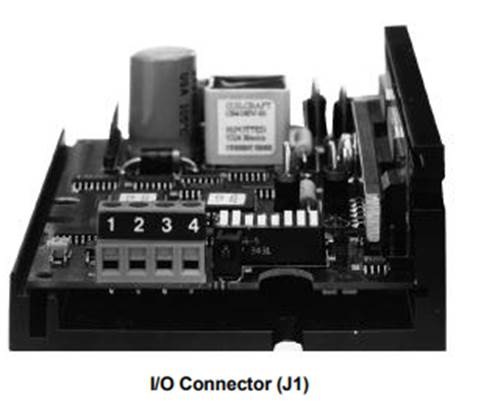
\includegraphics[scale=0.5]{./Figure/fig_steppermotorj1}
\caption{Figure of connection port J1 of the stepper motor driver.}\label{fig_stepmotorj1}
\end{figure}

\begin{figure}[h!]
\centering
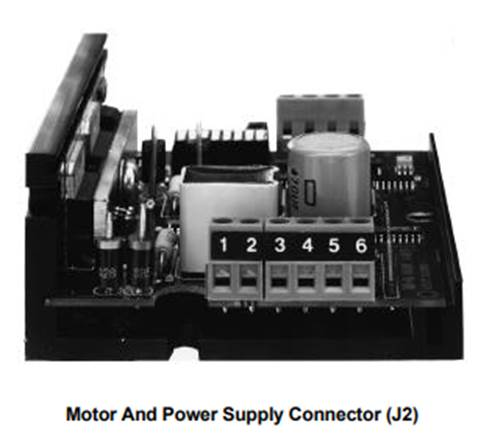
\includegraphics[scale=0.5]{./Figure/fig_steppermotorj2}
\caption{Figure of connection port J2 of the stepper motor driver.}\label{fig_steppermotorj2}
\end{figure}

The connection map is shown in the Table. \ref{tab_steppermotordriver}. The Pin 6 of J1 includes the \textbf{ground wire from the power supply as well as the GND wire from the myRio kit}. The VDD(5V) of J2 is connected to the 5V output on the myRio kit. 

\begin{table}
\centering
\caption{Table of the the stepper motor driver.}\label{tab_steppermotordriver}
\begin{tabular}{l|l|l}
\hline
\multicolumn{3}{c}{Team sheet}\\
\hline
Port number & Pin & Connection\\\hline
\multirow{6}{*}{J1} & 1 & motor 1\\
& 2 & motor 2\\
& 3 & motor 3  \\
& 4 & motor 4  \\
& 5 & VCC (24V)  \\
& 6 & GND \\\hline
\multirow{4}{*}{J2} & 1 & VDD(5V)\\
& 2 & DIO 3\\
& 3 & DIO 2\\
& 4 & DIO 1\\\hline
\end{tabular}
\end{table}
 
The stepper motor is controlled through a Labview MyRio kit. To run the Labview code to control the step motor, there are several steps:

\begin{enumerate}
\item Connect the power for the Labview MyRio. Connect the USB cable to the Windows desktop. 
\item Open the Labview and open the project. 
\item Run the Labview function by pressing the ``run" button (a white arrow).  
\item Turn on the power supply power. It should be noticed that \textbf{the power supply power should be opened only after the Labview is running}. Otherwise it might burn the motor. The current of the power supply should be less than 0.1 Amps. If the current is larger than 0.5 Amps and the motor is not spinning, it indicates something wrong and the power supply should be turned off immediately. 
\item Operate the front panel of the Labview. The front panel includes two pages. The first page is the single direction motion as shown in Fig. \ref{fig_labviewfront}. There are one switch for the direction, one switch for on/off and one knob for speed. The value on the knob is the command frequency of the motor, it does not mean the speed of the motor. Even though a larger frequency number moves the motor faster.  The second page (as shown in Fig. \ref{fig_labviewback}) is used to generate the sinusoidal motion. There are several rotating inputs that accept the angular frequencies and amplitudes input.
\item After the experiment is finished, \textbf{turn off the power supply first} and then quit the Labview.  
\end{enumerate}


\begin{figure}[h!]
\centering
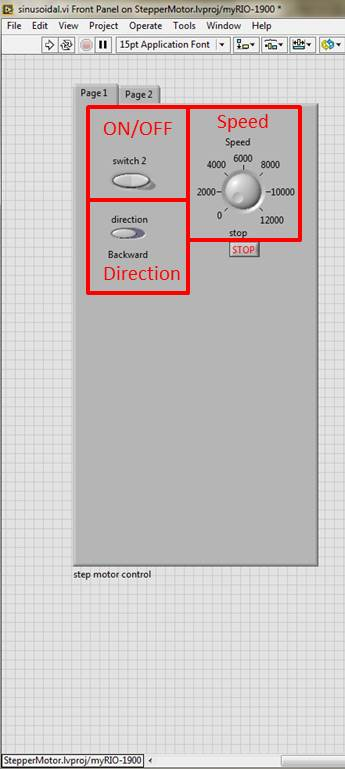
\includegraphics[scale=0.5]{./Figure/fig_labviewfront}
\caption{Figure of the front panel view of labview.}\label{fig_labviewfront}
\end{figure}

\begin{figure}[h!]
\centering
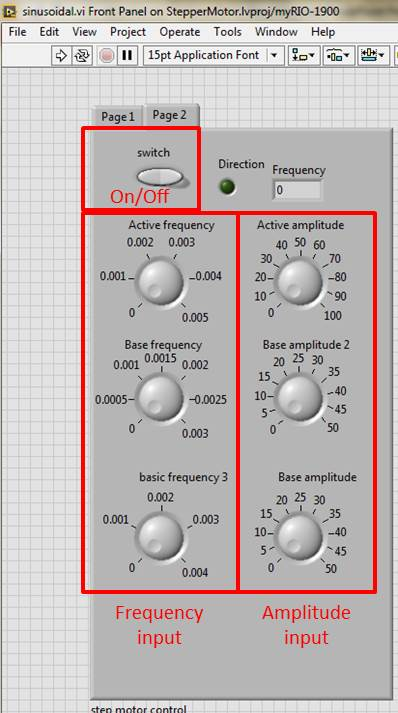
\includegraphics[scale=0.5]{./Figure/fig_labviewback}
\caption{Figure of the back panel view of labview.}\label{fig_labviewback}
\end{figure}


\chapter{MAV}
The MAV is a self-built autonomous hover quadrotor platform. The major sensors on the quadrotor include a MPU6050 gyro/accelerometer sensor, an optical flow sensor and a time-of-flight sensor. 


To fly the MAV, it also needs the motion capture, computer and the MAV itself. The computer and the motion capture system has been introduced in the previous chapter, this section will mainly focus on the MAV itself. 

\section{Flight controller connection}

This section will describe the connection of the flight controller as shown in Table. \ref{tab_wiremap}. 


\begin{table}[h!]
\centering
\caption{Table of the connection map.}\label{tab_wiremap}
\begin{tabular}{l|l|l}
\hline
Pin & Connection & Comment\\\hline
PB3 & LED & Green LED\\\hline
PB4 & LED & Red LED\\\hline
PA9 & UART1TX & Zigbee \\\hline
PA10 & USART1RX & Optical flow \\\hline
PA2 & USART2TX & \ \\\hline
PA3 & USART2RX & Zigbee \\\hline
PB10 & I2C1 SCL & TOF sensor\\\hline
PB11 & I2C1 SDA & TOF sensor\\\hline
PA8 & PWM1 & yellow wire\\\hline
PA11 & PWM2 & purple wire\\\hline
PB6 & PWM3 & red wire\\\hline
PB7 & PWM4 & white wire\\\hline
\end{tabular}
\end{table}
\section{Flight controller code}

Currently the code on the flight controller is written in C and compiled with the Keil $\mu$Vision software using the MDK ARM toolchain. The software can be downloaded from \url{https://www.keil.com/download/product/}


To flash the chip, there are several steps:

\begin{enumerate}
\item Open Google Chrome and search ``CleanFlight".
\item Add ``CleanFlight Configurator" to the Chrome APP.
\item Click on ``Firmware Flasher" and Select ``Load Firmware [local]".
\item Open the hex file in the \url{12_OpticalFlow_TOF_MAV/Objects} folder.
\item Use a jumper wire that connects the bootloader pad of the chip and 3.3V of the chip as shown in Fig. \ref{fig_flightcontroller}. The bootloader pad that needs to be connected to 3.3V is circled with a green box. 
\item Connect a micro USB cable with the chip and the computer. If the connection is correct, the chip will be in the bootloader mode. In this mode, only a blue LED indicates the power will be turned on. No other LEDs will be on or flashing. It is also important to \textbf{remove any wires on the USART1 pins} otherwise the flashing process will fail. The USART1 pins are shown in Fig. \ref{fig_flightcontroller}. 
\item Click on ``Flash Firmware" on the ``Cleanflight Configurator" app and wait until the flashing is finished.
\end{enumerate}

\begin{figure}
\centering
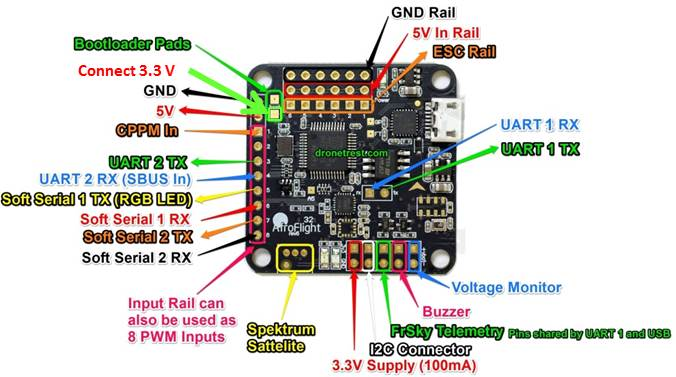
\includegraphics[scale=1]{./Figure/fig_flightcontroller}
\caption{Figure of the flight controller. }\label{fig_flightcontroller}
\end{figure}

\section{Optical flow code}
The Optical flow sensor can also be flashed. The compiling of the code is done on the Linux machine. The original code can be downloaded from the Github website \url{https://github.com/PX4/Flow}.


The instruction to flash the chip using the original code or the current code can be summarized as follows:

\begin{enumerate}
\item To build the project, enter the following command:
\begin{lstlisting}[language=bash]
>>make archives - this needs to be done only once
>>make
\end{lstlisting}
\item To flash via the PX4 bootloader (first run this command, then connect the board), enter the following command:
\begin{lstlisting}[language=bash]
>>make upload-usb
\end{lstlisting}
\end{enumerate}

\subsection{Frequent questions}

\begin{enumerate}
\item There a warning saying that the compiler version is not correct
\begin{lstlisting}[language=bash]
Unsupported version of xx found,  instead of one in 4.7.4 4.7.5 4.7.6 4.8.4 4.9.3 5.4.1
\end{lstlisting}

Answer: It is because an incorrect version of the gcc-arm toolchain is installed. One simple way to avoid the problem is to direct to the folder \url{/Flow/makefiles/baremetal/toolchain_gnu-arm-eabi.mk} and add the version of the gcc-arm-eabi-toolchain to the end of the following line:
\begin{lstlisting}[language=bash]
CROSSDEV_VER_SUPPORTED	 = 4.7.4 4.7.5 4.7.6 4.8.4 4.9.3 5.4.1
\end{lstlisting}

\item The flashing is not successful and it keeps displaying the following command:
\begin{lstlisting}[language=bash]
attempting reboot on /dev/ttyACM0...
\end{lstlisting}

Answer: It is because the flash is not in the bootloader mode. The approach is to press a button on the optical flow sensor and it will begin to flash.
\item How to adjust the focus of the optical flow sensor?

Answer: To adjust the focus of the optical flow sensor, there are several steps:
\begin{enumerate}
\item Flash the optical flow sensor with the original code. It should be noticed the original code is not compatible with the flight controller. 
\item Download the ``QGroundControl" from \url{http://qgroundcontrol.com/} and install the file. 
\item Open the ``QGroundControl" software. If the driver has been installed successfully, the software will automatically connect the sensor. 
\item Click on the second icon and the PX4Flow, a video will be displayed as shown in Fig. \ref{fig_qground}. From the video, the focus of the sensor can be adjusted. 
\end{enumerate}
\begin{figure}[h!]
\centering
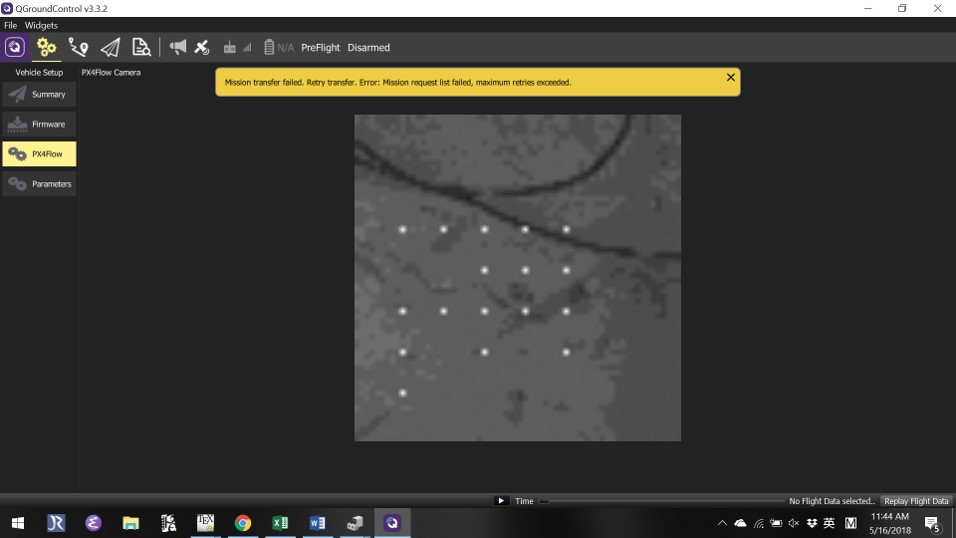
\includegraphics[scale=.4]{./Figure/fig_qground}
\caption{Figure of the QGroundControl software. A view from the camera can be displayed.}\label{fig_qground}
\end{figure}
\item What if the driver is not successfully installed as shown in Fig. \ref{fig_driver}?

\begin{figure}[h!]
\centering
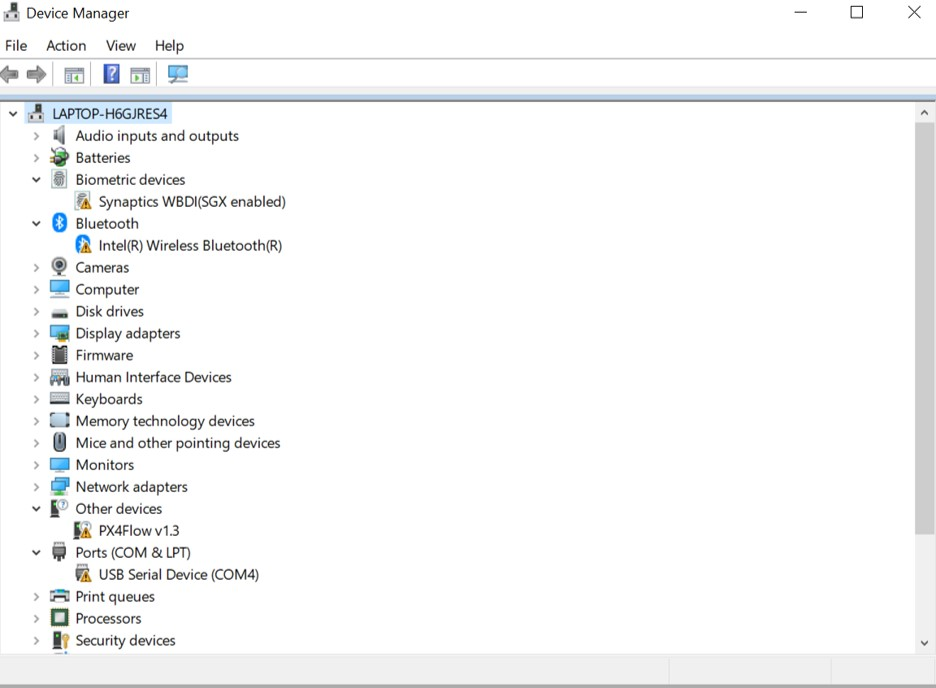
\includegraphics[scale=0.4]{./Figure/fig_drivers}
\caption{Figure of the driver installation problem for the PX4Flow sensor.}\label{fig_driver}
\end{figure}

Answer: Open the Device Manager, Right click on the ``PX4Flow V1.3" driver and click on ``Update driver". In the new popped out Window, select ``Browse my computer for driver software" and select ``Let me pick from a list of available drivers on my computer". Select ``Ports (COM $\&$ LPT)" and  select ``3DR Robotics". Click on ``PX4 Flow" and ``Next". The driver will then be installed. 
\end{enumerate}

\chapter{Ardrone}
The Ardrone is an off-shelf, cheap and reliable flying platform. The Ardrone is mainly used in Zhe's research. The Ardrone is equipped with onboard stabilized controller, optical flow sensor and ultrasonic sensor. By default, the Ardrone can stabilize itself in the hover. 

The Ardrone can also be controlled by Linux/Windows desktops through UDP connection. This chapter birefly introduces the procedure oto control Ardrone. 


The Ardrone is controlled through UDP port 5556. 

\begin{lstlisting}[language=Matlab]
ardroneUDP = udp('192.168.1.1', 5556, 'LocalPort', 5556);
fopen(ardroneUDP);
\end{lstlisting}

By sending different command through the UDP port, the Ardrone can take off/land/perform different maneuver. 


The control command includes the vertical speed, the roll, pitch angles and the yaw rate. A detailed explanation of the control command can be found in the Ardrone SDK manual. 



\section{Ardrone Wireless control}

There are several steps to control the Ardrone:

\begin{enumerate}
\item Turn on the power of the Ardrone. The LEDs on each of the Ardrone supporting legs should be green. 
\item Use motion capture to capture the markers on the Ardrone. If no markers are installed, install the markers first. 
\item Connect to the Wifi. Based on different Ardrones, the WiFi address will be different. The correct WiFi ID should be similar to ``Ardrone2$\_$ ..." or ``Ardrone$\_$...".
\item Run the Matlab code to test the Ardone. Use the joystick to control the maneuver of the Ardrone. 
\end{enumerate}
\chapter{Useful tools}

This chapter introduces several very useful tools which will greatly improve the productively in my opinion for a PhD student. 
\section{Jabref}
This is a reference management tool. It is compatible with the bibtex. One big challenge is that it is very difficult to find several PDF files with same key words. With this software, it is easy to associate PDF files with key words and hypelinks.  An example of the Jabref can be found in Fig. \ref{fig_jabref}. 


\begin{figure}[h!]
\centering
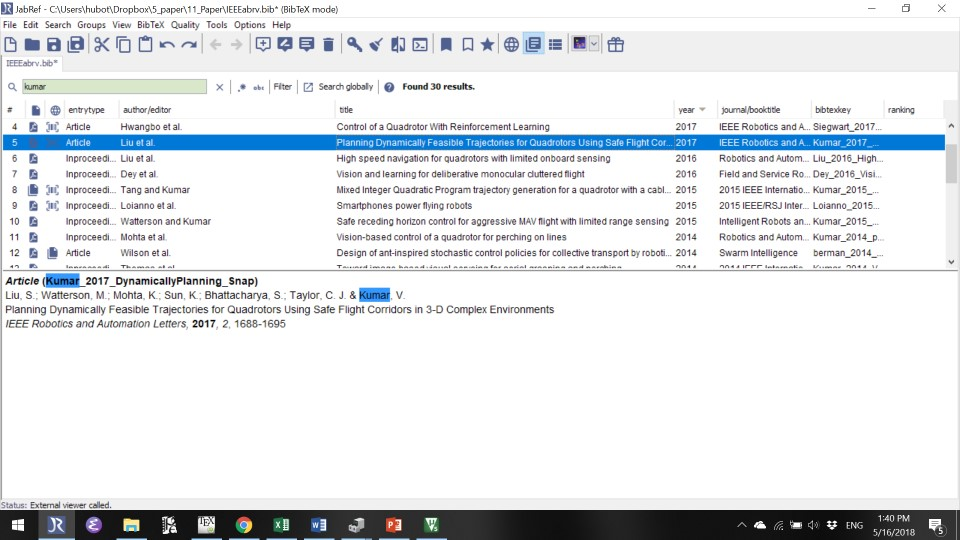
\includegraphics[scale=0.5]{./Figure/fig_jabref}
\caption{Figure of the Jabref software.}\label{fig_jabref}
\end{figure}



\begin{enumerate}
\item Download the software from the website: \url{http://www.jabref.org/}.
\item Open the software and click on ``Open BixTex Database" if you already have some bibtex file. 
\item Click on  ``New bibtex entry" and select the type.
\item Click on ``Bibtex source" and paste in the bibtex source information. These information can usually be downloaded from Google or IEEE website.
\item Change the caption to be a preferred format. My personal favorite format is ``Name$\_$Year$\_$Key words" such as ``Kumar$\_$2017$\_$AutonomousFlying".
\item Save the PDF file to be the same name under the same root as the bibtex database file.
\item Click on ``General" and ``Get fulltext". The PDF file will be associated with this bibtex entry. A PDF icon will be displayed before the bibtex entry. The next time you want to see the PDF, you can just view it from the Jabref software by clicking the  PDF icon.
\end{enumerate}

\section{STM32CubeMX}
The STM32CubeMX is a software that provides project templates for STM32. The STM32CubeMX is based on the HAL (High-level Abstract Library). Current STM32 project is based on STM32 Standard Peripheral Library (SPL). The advantage of using HAL over SPL is that the SPL is no longer supported in the future. 
 
The software can be downloaded from ST website: \url{http://www.st.com/en/development-tools/stm32cubemx.html}. The download link is at the bottom of the page. 

There are various video tutorials about how to use the software. An example can be found at \url{https://www.youtube.com/watch?v=imXauCiwEfs}.  



\end{document}

